\documentclass{article} % For LaTeX2e
\usepackage{nips14submit_e,times}
\usepackage{hyperref}
\definecolor{linkcolour}{rgb}{0,0.2,0.6} % Link color
\hypersetup{colorlinks,breaklinks,urlcolor=linkcolour,linkcolor=linkcolour} % Set link colors throughout the document
\usepackage{graphicx}
\usepackage{url}
%\documentstyle[nips14submit_09,times,art10]{article} % For LaTeX 2.09


\title{In the Arena of Neural Nets Optimizations}


\author{
Junbo Zhao \\
Center of Data Science\\
New York University\\
\texttt{j.zhao@nyu.edu} 
}

% The \author macro works with any number of authors. There are two commands
% used to separate the names and addresses of multiple authors: \And and \AND.
%
% Using \And between authors leaves it to \LaTeX{} to determine where to break
% the lines. Using \AND forces a linebreak at that point. So, if \LaTeX{}
% puts 3 of 4 authors names on the first line, and the last on the second
% line, try using \AND instead of \And before the third author name.

\newcommand{\fix}{\marginpar{FIX}}
\newcommand{\new}{\marginpar{NEW}}

\nipsfinalcopy % Uncomment for camera-ready version

% Add by Jake
\usepackage{amsmath,amsfonts,amssymb}
\newcommand\transp{^\intercal\kern-\scriptspace}

\begin{document}


\maketitle

\begin{abstract}
If we leave alone the topography of Neural Net, it could be regarded as a model that consists of several different nonlinear and linear mappings; it distorts and stretches the initial space consecutively and ends up with projecting the points to the right places. The error surface (equivalent to the loss function contour w.r.t the weights) is intractable and fairly complicated; that is, in general it is nonconvex and involves many local minimums. Stochastic Gradient Descent is the most predominant methodology, usually assisted by Momentum and Adaptive step sizes. Meanwhile, Quasi-Newton methods, such as BFGS and Levenberg-Marquardt Algorithms are still widely applied. Furthermore, Conjugate information gives rise to Conjugate Gradient method, which simplifies training significantly. In this article, we investigate and compare different methods of different settings on optimizing Auto-encoder, a fully-connected associated Neural Net. The Numerical issue found during training is also presented and analyzed.
\end{abstract}

\section{Introduction}
Neural Net literature has a long history with lots of scientific researches in the past 50 years. It was originally invented in 1960s. The first hot trend happend two decades later, in 1980s when Multilayer Perceptron (MLP) was created, Neural Nets made the world believe Artificial Intelligence was incoming. But unfortunately, this trend faded away soon due to the difficulty of training, as well as the invention of Support Vector Machine (SVM) and Boosting. 

Differing from Neural Nets, SVM and Boosting are both statistical methods, benefiting from solid theoretical foundation. Some tricks are specifically designed for optimizing SVM and Boosting which was proved to be very effective. Compared to these fancier and more sophisticated models, the winter of Neural Nets came.

However, upon the astonishing results in ImageNet Challenge [1] produced by Deep Learning, Neural Net confidently announced its coming back. ImageNet [2] is one of the mostly well-known competitions in Computer Vision. The challenge involved different tasks such as object recognition and detection. With the giant dataset and attentive classifications, the best result prior to 2012 was only 74\% on classification challenge. Nevertheless, Krizhevsky et al. [1] made a big enhancement to 85\%, and won the competition in 2012. More amazingly, the state-of-the-art was further improved to nearly 90\% in 2013, by Zeiler et al. [3], where the Deep Learning was employed as well. After enduring the winter for a decade, Neural Net made a big bounce back. Essentially its coming back was mainly owing to fitting much more data in a deeper and more giant Neural Net, and trained by modern GPU or some other parallel computing systems.

For Optimization purposes and advocated by the mania of Deep Learning, many methods that are able to reduce the training time are proposed nowadays. Unlike traditional optimization methods, the optimization used for Deep Learning is always short up rigorous convergence prove, but greatly relies on the experimental results. Asynchronous Stochastic Gradient Descent is one of the most popular examples[4]. The parallel system in [4] constructs a parameter “server”, which gives replicas parameters and updates the parameters stored periodically , i.e. in a asynchronous manner. This will make Optimization people very unsatisfied because training process uses neither up-to-date weights nor the real gradient to make an update. In particular, the gradients are always out-of-date that might deviate the optimizing route. However, modern Machine Learning has to sustain the tradeoff between converging speed and the errors like this.

Second order methods, such as L-BFGS and Levenberg-Marquardt methods are still applied. But the reason why they are less prevalent than SGD nonetheless is due to the "batch" nature of these methods. In each epoch, they have to visit the whole dataset. When the dataset is relatively large, they may perform slowly. From Optimization perspective, they might be able to converge in less epoches. But in fact it may require more time since each epoch takes longer time to compute the entire dataset. Machine Learning people usually prefer "shorter time" to "less epoches".

Neural Net training has Numerical issues. Ill-conditioning is detrimental in most cases. Ill-posed training always deals with a distorted error surface, whereby flatness occurs in many right directions (point to minimum) but it can be highly curved in some other wrong directions. If trapped in these kinds of directions, optimization always has to take a lengthy detour. This part will be discussed in Section 4. In addition, Machine Learning people sometimes hold different point of view on ill-conditioning.

The article is organized as following: Section 2 briefly describes the model Auto-encoder, which is an associated Neural Net as our benchmark model. Section 3 illustrates a few optimization algorithms and most of them are tested in our experiments. Section 4 is devoted to a practical observation on experimental results. Section 5 makes some further discussion.


\section{Sparse Auto-encoder}
\subsection{Auto-encoder}
Auto-encoder is an associated (Output target simply replicates the input) Neural Net, which lets the Neural Net form a good reconstruction of the input by itself. The Auto-encoder is mainly used to automatically extract the features from unlabelled data, i.e. in an unsupervised manner. For simplicity, we employ an Auto-encoder with three layers, between which a nonlinear mapping is placed, known as "sigmoid" activation function:
$$
\sigma(x) = \frac{1}{1+e^{-x}},
$$
which apparently lies between 0 and 1, shown in Figure 1.

Given the skeleton of this model, we can write down the loss function, i.e. objective function of Optimization purpose, as:
$$
\min_{W, b} \quad \sum_{i=1}^m \| \sigma( W^{(2)} \sigma( W^{(1)} x^{(i)}+b^{(1)} )+b^{(2)} )-x^{(i)} \|_2^2,
$$
where we use the standard least square model that directly measures how well the model reconstructs the input. Note that $W{(l)}$, $b{(l)}$ respectively denote the weights and bias of layer $l$ (our training targets), and $x{(i)}$ denotes the $i_{th}$ sample in the training dataset.


\subsection{Sparse penalty}
Sparsity is a commonly used word in Machine Learning community. Imposing sparsity on Neural Net model training is usually highly recommended. The reason for this is that Neural Net often overfits easily, i.e. yielding a very low loss on training set but performing badly when fitting test samples in the trained model. This is also known as the "generalization capacity". The sparsity penalty nonetheless drives Neural Net to learn much concentrated and effective features, by being restricted to only use a few alive neurons to reconstruct signal. In this sense, overfitting can usually be alleviated.

To be specific, the trick is to manually set a constraint on the hidden layer activations:
$$
\rho_i = \rho,
$$
where $\rho$ is the sparsity constraint target and $\rho_i$ denotes the $i_{th}$ activation of the hidden layer:
$$
\rho_i = \sigma(\sum_j W_{ij}^{(1)} x + b_i^{(1)} ).
$$
Usually, we may set the target value $\rho$ to a very small number, such as 0.0001. Similar to Penalty function method, we may convert this constraint optimization problem to unconstrained optimization, by adding a term that penalizes the difference between the real activation and this sparse target. We apply K-L divergence:
$$
P = \sum_i{\rho \log \frac{\rho}{\rho_i} + (1-\rho) \log \frac{1-\rho}{1-\rho_i} }.
$$
Now we have derived the entire loss function for Sparse Auto-encoder: 
\begin{align*}
\min_{W, b} \quad & \sum_{i=1}^m \|	 \sigma( W^{(2)} \sigma( W^{(1)} x^{(i)}+b^{(1)} )+b^{(2)} )-x^{(i)} \|_2^2 \\
&\quad \quad \quad  + \lambda_1 [\sum_i{\rho \log \frac{\rho}{\rho_i} + (1-\rho) \log \frac{1-\rho}{1-\rho_i} }] \\
& \quad \quad \quad + \lambda_2 [\sum_{i,j,l} (W_{ij}^{(l)})^2],
\end{align*}
where the last term is "weight decay", another frequently used term for preventing overfitting. By taking a brief look at the loss function, we could figure out its complexity: it is non-convex. The dimension of concatenated weights (obtained by concatenating $W^{(l)}$ as well as $b^{(l)}$ which are our targets of optimization) reaches $10^4$. Hessian, or pseudo Hessian approximated by Quasi-Newton methods, would be nearly $\mathbb{R}^{10^4 \times 10^4}$. When curvature is involved, computation would become extremely expensive.

After optimization we could visualize the weight $W^{(1)}$ to see what the model learns. Some visualization results, trained by different methods, are displayed in Figure 2.\\
\begin{tabular}{ccc}
    \includegraphics[width=0.3\columnwidth]{img/sigmoid.png}  &
    \includegraphics[width=0.3\columnwidth]{img/RELU.png} &
    \includegraphics[width=0.3\columnwidth]{img/shrink.png} \\
    (a) & (b) & (c)
\end{tabular}
{\bf Figure 1} Different activation functions: (a) sigmoid; (b) rectified linear; (c) shrinking

\begin{tabular}{cc}
    \includegraphics[width=0.5\columnwidth]{img/bfgs.jpg}  &
    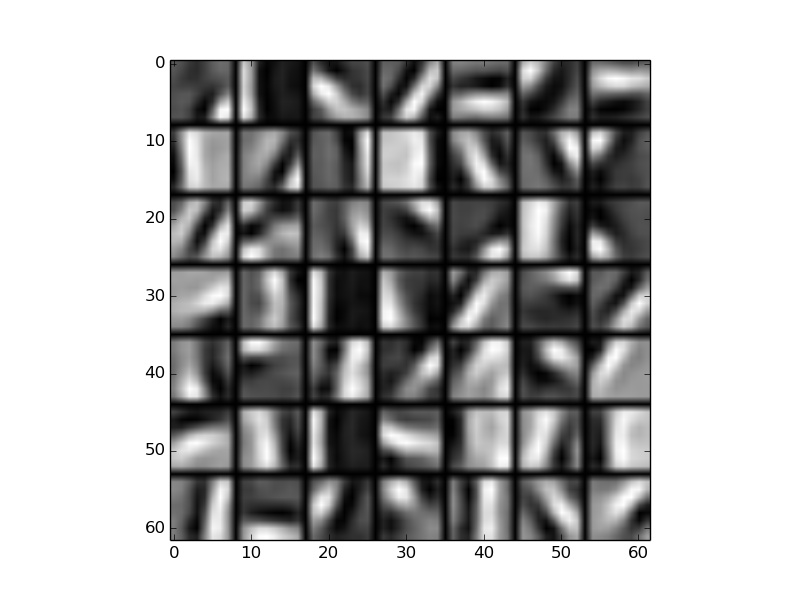
\includegraphics[width=0.5\columnwidth]{img/cg.jpg} \\
    (a) & (b)
\end{tabular}

\begin{center}
\includegraphics[width=0.5\columnwidth]{img/sgd.jpg} \\
(c)
\end{center}
%\begin{center}
% \includegraphics[width=0.5\columnwidth]{img/bfgs.jpg}  \\
% (a)\\
%    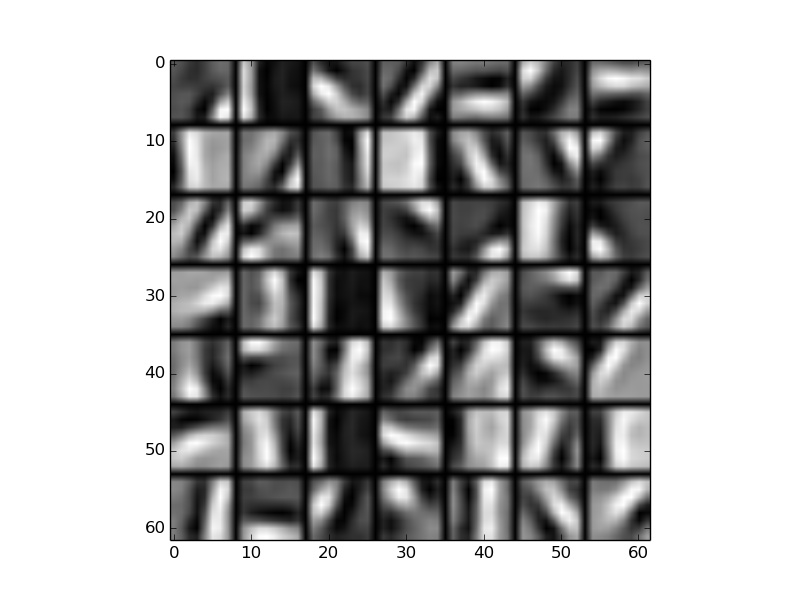
\includegraphics[width=0.5\columnwidth]{img/cg.jpg} \\
%    (b) \\
%    \includegraphics[width=0.5\columnwidth]{img/sgd.jpg} \\
%    (c)
%\end{center}
{\bf Figure 2} Auto-encoder learns in the hidden layer, i.e. low level representations in the images (edges or corners): (a) learned by BFGS; (b) learned by CG; (c) learned by SGD.

\section{Methods}
\subsection{Stochastic Gradient Descent}
SGD is predominantly employed in Neural Net training [5]. It is always fast, easy to implement or interpret. Since the gradients are generated from samples stochastically chosen from the dataset, it is less likely to fall into local minimum comparing to the primitive batch Gradient descent. Besides, SGD allows lots of flexibility; it allows dataset dynamically changing, i.e. On-line learning that is able to merge new data in the dataset. This also gives rise to asynchronous SGD as we have illustrated before.

However, we have to point out that SGD has lots of disadvantages. More importantly, SGD always requires much manual tuning. It does not perform stably well, in particular when using Momentum without line search. Sometimes with bad parameters setting, SGD can perform poorly [5].

Several tricks are proposed to enhance stability of SGD:
\begin{itemize}
   \item {\bf Momentum}. This trick is always applied in Neural Net training:
   $$
   \Delta w(t+1) = \beta \frac{\partial L_t}{\partial w} + \mu \Delta w(t),
   $$
   where $\beta$ denotes current step size and $\mu$ denotes Momentum term. When the error surface is complicated that has different curvatures toward different directions, error surface would resemble some long and narrow valleys, i.e. dangerous local minimums. Momentum is adopted to overcome this potential hazard and it works to drive the steps go across the "valleys".

   \item {\bf Adapgrad}. The step size has to be reduced. 
In an extreme case, when we apply conventional gradient descent method and are almost very close to the minimum, big step size would definitely go back and forth with respect to the minimum, and this could even spoil previous efforts. Hence, gradually reducing the step size is always deemed as a must when performing SGD.

   There are so many methods proposed based on this idea. The simplest one should be $ \beta = \frac{\beta_0}{C+t} $, where $C$ is a constant and $t$ is the time elapsed. This is very straightforward that reducing the step size gradually, along with the increasing elapsed time. More complicated one should be "Adagrad" [12]:
   \begin{align*}
      w_{t+1}^i &= w_{t}^i - \eta^i_t \frac{\partial L_{t}}{\partial w^i_t} \\
      \eta^i_t &= \frac{\eta}{\sqrt{\sum_{s=1}^t (\frac{\partial L_t}{\partial w^i_t})^2}}.
   \end{align*}
   As we can see, this method is operated in a component-wise fashion. Each parameter has its own adaptive learning rate and each of them are adapting to the component. Adagrad is often used along with Momentum; that is Adagrad gently and meticulously anneal the learning speed while Momentum strongly speeds it up along the directions. The mixture seems very interesting [13].

   \item {\bf Mini-batch} This method mainly attacks some non-differentiable activated Neural Net. Basically traditional SGD only picks one sample to yield gradient in one iterate, and finishes using all the samples in an epoch. Mini-batch SGD nevertheless picks a bunch of samples in an iterate, and visits all the training samples once in one epoch. The extreme Mini-batch SGD is Batch Gradient Descent. 

   Mini-batch SGD is often adopted when the activation function is not differentiable at some specific points (see once again the gap between Optimization world and Machine Learning world), such as rectified linear and shrinking function, shown in Figure 1 (b, c). This is because in this case, only pick one sample could happen to be non-differentiable. Typically if using an approximated gradient to generate step, this is potentially taking risk of going farther away from minimum. However, Mini-batch operates on a small bunch of samples, aiming at reducing the negative effect of the approximated gradients from some non-differentiable points. This method looks rather horrible for Optimization people since this could never be proved rigorously, even asymptotically. But actually Machine Learning people always use this when performing SGD.

   Note in our experiments where "sigmoid" is differentiable for entire $x$ domain,  Mini-batch training may not be useful. We discuss more in Section 4.
\end{itemize}

\subsection{BFGS}
As we all know, BFGS involves curvature. Using Backpropogation [7, 8] renders a quick approach to derive the gradients of the loss function with respect to the weights that is targeted to learn. The weights are always high dimensional that making Hessian intractable. BFGS approximates Hessian starting from a symmetric matrix. For Machine Learning purposes, second order information, known as curvature in Optimization, is often regarded as modeling the interaction between the variables.

The extension of BFGS is the Limit Memory BFGS. But unfortunately as time is constrained, we haven't investigated the capacity of L-BFGS which could be faster and resolve the storage worries. 

The weakness of BFGS is that it has to compute through the entire training dataset for that each iteration, i.e. a batch method. Also, it strongly relies on the speed of libraries. Worse yet, a step either computing the inverse of the approximated Hessian or solving a huge linear system is inevitable in each BFGS update. This step could be extremely slow (Specific comparison could be seen later), in particular running by scripting language (such as Python). On the contrary, using C or Fortran can speed it up; but this could still be one of the bottlenecks of BFGS.

\subsection{Levenberg-Marquardt}
Referring to the course Note 11 [9], Levenberg-Marquardt is explained by an improvement on Gauss-Newton method, which keeps the approximated Hessian always positive definite. Levenberg-Marquardt effectively solves the ill-conditioning in $(J_k \transp J_k)^{-1} $ by raising the singular value of trivial magnitude.

Meanwhile, Levenberg-Marquardt can be explained from Machine Learning perspective. L-M is always regarded as the combination of steepest descent and Gauss-Newton method [10]. To get started, we have 
$$
(J_k \transp J_k + \sigma I)s_{\sigma} = -J_k \transp F_k,
$$
whereby we can present it as
$$
w_{k+1} = w_k - (J_k \transp J_k + \sigma I)^{-1}J_k F_k.
$$
In the sense, when the manually set parameter $\sigma$ is very small and the function has very well-posed, L-M update reduces to Gauss-Newton method. On the other hand, when $\sigma$ becomes large, meaning the second order information is much ill-conditioned, L-M resembles steepest descent where $\frac{1}{\sigma}$ is the learning step size [10]. Thus we can conclude L-M updates alternate between steepest descent and Gauss-Newton method. This method implicitly combines these two methods in order to pursue fast convergence and keep it stable at the meantime. There is somehow a resemblance between L-M and Brent's method [11] in one dimensional zero finding, which explicitly combines different methods (L-M implicitly).

Furthermore, Matlab is known as numerical computing. we conjecture that the reason why Neural Net toolbox has a L-M optimization is that it has numerical stability. The alternating procedure would achieve fast steps by performing Gauss-Newton updates and falls back to steepest descent when the approximated Hessian is ill-conditioned, which indicates the bad condition of the curvature. Thus, L-M is much more immune to Numerical problems.

\subsection{Conjugate method}
Conjugate gradient descent has been known as a misnomer, since for each update the directions are obviously not the one of gradients. A more precise name would be "Conjugated pseudo-gradient descent". Essentially, CG is always trying to avoid damaging the effort made in the previous iterates. CG could also be regarded as performing optimization in a spinned and stretched space from the initial one. In this space, performing orthogonal steps is equivalent with performing conjugated steps in the original space. The mapping is always changing in Neural Net training; that is because the mapping is decided by the curvature of error surface and the surface keeps changing during Neural Net training. Thus, in fact in the mapped space, CG is always reducing the residue toward the targets; but inversely it might not reduce the loss function seen from the original space. In this sense, CG is likely to fluctuate during training, but eventually it converges to the minimum. CG is also a batch method, which shares the weakness with BFGS. It has to visit every sample in order to make an update.

Specifically, CG is capable of adapting to the ill-conditioning spaces. More experimental results support this point of view is presented in Section 4.

\section{Experiments}

In this section, we present a bunch of experimental results of Auto-encoder training. The metric used is the value of loss function against {\bf time}, not epoch. Note temporal obsearvation is standard in Machine Learning. We compare optimization of different methods on different training scales. Since we are quite interested in SGD, we decide to test different settings, i.e. Momentum/Adagrad/Mini-batch. Numerical issue testing is another indispensable part which is discussed later in this section. We use server from Courant \texttt{crunchy6.cims.nyu.edu}, which has 4 AMD CPU cores at 2.1GHz, and all of the experiments are performed in Python.

\subsection{Set Up}
Auto-encoder is chosen as the targeted training model. Our experiments are carried out on a dataset of 25 gray images, which are crawled from Google and cropped to patches beforehand. Each cropped patch is of size 8*8, and all of pixel values are normalized to (0, 1) [14]. Thus, the size of input size of Auto-encoder is 64. The hidden layer size is set to be 49, aiming to supply the space of sparse representation. Auto-encoder is an associated framework and, therefore, the output layer is the same as input layer. The nonlinearity mainly comes from sigmoid activation equipped right before the signal going into the hidden layers and the output layers. Lastly, the sparsity target $\rho$ is chosen as 0.0001. Corresponded penalty term is 3.

The Auto-endoer is expected to learn the low level representations as Figure 2 shows. Taking a brief look in Figure 2, we can clearly see that low level representations yielded by BFGS or CG are slightly better than the one learned by SGD; that is, the figure visualized from the weights that learned by BFGS and CG looks very smooth, i.e. most of them display clean edges as expected. SGD performs well, but, obviously the figure it yields seems moderately noisy and less transparent.

For optimization purposes, we focus on how fast it converges to the minimum, i.e. how quickly the value of loss function decreases. All the plots posted afterward show loss function against time. The reason for not choosing "epoch" as the checkpoint could be that this measurement does not take into account the time each epoch needs, especially bearing in mind the weakness of batch methods such as BFGS and CG. In this sense, using loss function against time as the metric is very common in Machine Learning community. This might be another difference between the two communities.

\subsection{Training Scale}
The training samples are all 8*8, vectorized as 64 dimension. In this experiment, we propose to gradually increase the number of training samples, i.e. scale, to compare BFGS, CG and SGD. Results are presented in Figure 3 below. \\
    \begin{tabular}{cc}
    \includegraphics[width=0.5\columnwidth]{img/scale/1.png}  & \includegraphics[width=0.5\columnwidth]{img/scale/2.png} \\
    (a) & (b) \\
    \includegraphics[width=0.5\columnwidth]{img/scale/4.png}  & \includegraphics[width=0.5\columnwidth]{img/scale/6.png} \\
    (c) & (d) \\
    \end{tabular}
    {\bf Figure 3}. Optimization comparison of different training set scale: (a) 10000 samples; (b) 20000 samples; (c) 60000 samples; (d) 102400 samples. We fix the range of $x$-axis as \texttt{[0,100]} and $y$-axis as \texttt{[0,20]} in order to takes close look at the convergence when optimizer is close to the minimum. \\
    
In the training process, it is likely that SGD and BFGS are both faster than CG, which fluctuates all the time on the non-convex error surface. For the comparison between BGFS and SGD, we propose to use the \textbf{area} between two optimizing curves in order to see the difference. Since graphs often have fixed range of axis \texttt{xlim=(0,100), ylim=(0,20)}, we could directly compare the area in the figure without worrying about zooming; along with the increasing sizes of training set, we could derive that the advantages of BFGS decreases and even vanishes in (d), which trains on the largest scale training set. This is accorded to our expectation that the weakness of batch method will be revealed when dataset becomes larger.

\subsection{Blend of Adagrad and Momentum}
In this section, We investigate whether Adagrad and Momentum applies. As we have discussed, Momentum and Adagrad, which are two seemingly contradicted powers, could be an interesting mingle. In practice, they can cooperate with each other to benefit optimizing. This is shown in Figure 5.\\
\begin{center}
\includegraphics[width=0.5\columnwidth]{img/ada/1.png} 
\end{center}
{\bf Figure 4}. As legend shows, "ada" means applying Adagrad while "Nada" is on the contrary that Not applying Adagrad. The successive "95" means using \texttt{.95} as Momentum term used. Training is performed on a dataset of 40960 samples. To take a close look, we set \texttt{xlim=(4,50), ylim=(0,5)}.\\

Interestingly, we could make multiple comparisons here. From (green, yellow) we conjecture that without the constraint of Adagrad an a "rein", 0.95 Momentum (with line search) is in fact deleterious. Group (red, blue) reveals the blend of Momentum and Adagrad behaves better than solely adopting Adagrad without Momentum as a "darting horse". Furthermore (red, green) tells that without Momentum, Adagrad seems not doing any favor; and (blue, yellow) in its turn emphasizes the importance of this mixture. In a word, the blue line, which is the optimal, indicates that a mild blend of Momentum and Adagrad eases optimization.

\subsection{Mini-batch}
In this section, we focus on the application of Mini-batch method for SGD. Intuitively, since "sigmoid" as the activation function, which is rather smooth and stable, importantly differentiable at all spots, Mini-batch may not be useful. This is shown in Figure 6.
\begin{center}
\includegraphics[width=0.5\columnwidth]{img/mb/1.png} 
\end{center}
{\bf Figure 5}. Comparisons on different Mini-batch settings. The number in the legend tells the size of Mini-batch applied. Experiments are performed on training set, which consists of 102400 samples. Momentum and Adagrad are all applied.

As expected, Mini-batch does not apply. From the figure, there isn't strong correlation between the size of Mini-batch and the execution of SGD. Additionally, training without Mini-batch even performs best. Hence, in our experimental settings, where a smooth "sigmoid" activation function is adopted, Mini-batch looks not so useful.

\subsection{Numerical issues} In this section, we intend to break the condition of training set by making it rank-deficient, and in its turn test the numerical stability of BFGS, CG and SGD. Fortunately, the three methods under this condition are all able to sustain converging, which is shown in Figure 6. However, we admit that in our settings ill-conditioning could not propagate much in a three-layer Auto-encoder, but it would propagate severely in deeper frameworks. We may leave this to future work.\\	
\begin{tabular}{cc}
    \includegraphics[width=0.5\columnwidth]{img/ni/sgd.png}  & \includegraphics[width=0.5\columnwidth]{img/ni/bfgs.png} \\
    (a) & (b) \\
    \includegraphics[width=0.5\columnwidth]{img/ni/cg1.png}  & \includegraphics[width=0.5\columnwidth]{img/ni/cg2.png} \\
    (c) & (d) \\
\end{tabular}
{\bf Figure 6}. Numerical stability testing on BFGS, SGD and CG. (a) SGD; (b) BFGS; (c) CG; (d) CG closer look. We fix the range of $x$-axis as \texttt{[0,100]} and $y$-axis as \texttt{[0,20]} in order to take close look at the convergence when optimizer is close to the minimum. The condition numbers of "good", "ill", "worse" and "worst" are 707, 4019, 44173, 4784347 respectively. \\

Starting with SGD, the smooth curve uncovers the robustness of SGD standing up ill-conditioning. But ill-conditioned error surface does slack the speed of SGD (with line search), as the yellow line converges slowest. BFGS also effectively adapts to the ill-conditioning, though in the worst case BFGS loses some speed.

CG looks more interesting. As we know before, CG may fluctuate during training and the experiments in Section 4 are all done in well-posed environment. From Figure 6(c) and 6(d), we know that under ill-conditioned circumstances, CG fluctuates more drastically, as shown by blue and green lines. Instead, the red line fluctuates mildly, while CG converges eventually however. 


\section{Discussion}
Numerical issue are always considered to be harmful and detrimental in Optimization community since it always damages the stability of algorithms and keeps them oscillating. But in Machine Learning community, it might not be the case. Let's go back to the definition of ill-conditioning, “small change of input renders large changes of output”. However, in Machine Learning world, input for optimization can be defined as the model and loss function. Targeted weights can be seen as outputs. In this sense, ill-conditioning is translated by that small changes in the model makes big difference of weights. Inversely, we can also say that not so accurate weights has little impact on the model and the objective function. This is a virtue that is always called "fault tolerance" in Machine Learning world.

Overfitting is another interesting topic of the marriage of Machine Learning and Optimization. Overfitting means that optimizing on the training set yields a very small minimizer of the loss function, but it performs rather poorly on the testing set. This is one of the most essential problems in Machine Learning world. However, for Optimization purposes, the rules are always like: the less minimizer can be obtained, the better models will be. In my understanding, this is one of the biggest gaps between the two worlds. In the training phase, Optimization is bent on getting a lower function value at optimal speed while sometimes Machine Learning has to stop it or even let it go back. A slightly higher function value is fatal in Optimization, but is acceptable for Machine Learning. The only benchmark to judge a Machine Learning algorithm is applied in the testing phase, not in the training phase. In a word, they have different purposes.

\newpage
\section*{Acknowledgement}
I would like to thank Professor Margaret Wright for providing all those useful materials and interesting topics in this course. Four months ago, I came to this campus with a sense of insecurity. Having travelled half way across the globe, I couldn't have felt more out of place. In my very first semester in the US, without fluent English and proficient writing skills, I felt somehow nervous to take the Numerical Optimization course. However, I now feel fulfilled and grateful because I made the right decision to take the course. Professor Margaret is always enthusiastic in her lectures and is also very patient during office hours, especially when answering my crappy questions. The moment I finished the last word of this report signifying the end of this short journey for me, I realized how far I have come and how much I have learned. From Margaret's elaborately prepared homework, I can still remember Klee-Minty, together with those interesting diet plans. For the best course I have ever taken, I would be excited to take more challenges in my future study!

\section*{Appendix}
All the code and plots are posted on my github: \\
\href{https://github.com/zhaojunbo/StarAE}{\bf Code} /  \href{https://github.com/zhaojunbo/StarAE/tree/master/test/optim_proj}{\bf Plots}

Git record: \texttt{36 commits / 6,456 ++ / 2,887 --}, in total \textbf{3569} lines of Python code.

\newpage
\section*{Reference}
\small{
[1] Krizhevsky, Alex, Ilya Sutskever, and Geoffrey E. Hinton. "Imagenet classification with deep convolutional neural networks." Advances in neural information processing systems. 2012.

[2] http://www.image-net.org/

[3] http://www.image-net.org/challenges/LSVRC/2013/results.php

[4] Dean, Jeffrey, et al.. "Large scale distributed deep networks." Advances in Neural Information Processing Systems. 2012.

[5] LeCun, Yann, et al.. "Gradient-based learning applied to document recognition."Proceedings of the IEEE 86.11 (1998): 2278-2324.

[6] Ngiam, Jiquan, et al.. "On optimization methods for deep learning." Proceedings of the 28th International Conference on Machine Learning (ICML-11). 2011.

[7] Rumelhart, David E., Geoffrey E. Hinton, and Ronald J. Williams. Learning internal representations by error propagation. No. ICS-8506. CALIFORNIA UNIV SAN DIEGO LA JOLLA INST FOR COGNITIVE SCIENCE, 1985.

[8] LeCun, Yann A., et al.. "Efficient backprop." Neural networks: Tricks of the trade. Springer Berlin Heidelberg, 2012. 9-48.

[9] Course Note 11.

[10] Yu, Hao, and Bogdan M. Wilamowski. "Levenberg-marquardt training." The Industrial Electronics Handbook 5 (2011): 1-15.

[11] Brent, Richard P. "An algorithm with guaranteed convergence for finding a zero of a function." The Computer Journal 14.4 (1971): 422-425.

[12] Zeiler, Matthew D. "ADADELTA: An adaptive learning rate method." arXiv preprint arXiv:1212.5701 (2012).

[13] Zeiler, Matthew D., et al.. "On rectified linear units for speech processing."Acoustics, Speech and Signal Processing (ICASSP), 2013 IEEE International Conference on. IEEE, 2013.

[14] Glorot, Xavier, and Yoshua Bengio. "Understanding the difficulty of training deep feedforward neural networks." International Conference on Artificial Intelligence and Statistics. 2010.
}


\end{document}
